\documentclass[presentation]{beamer}
\usetheme{Frankfurt}
\usecolortheme{default}
\title[Allele frequencies in autopolyploids]{Estimating allele frequencies in non-model [auto]polyploids using high throughput sequencing data}
\author[Blischak et al.]{Paul Blischak\inst{1}, Laura Kubatko\inst{1,2} and Andrea Wolfe\inst{1}}

\institute[OSU]{\inst{1}Dept. of EEOB\\  \inst{2}Dept. of Statistics \\ The Ohio State University}

\date{29 July, 2015}

\setbeamercolor{alerted text}{fg=blue}

\begin{document}

\begin{frame}[plain]
	\titlepage
	\vspace{-0.3in}
	\begin{center}
		
\includegraphics[width=0.25\textwidth]{fig/botany2015logo}
	\end{center}
\end{frame}

\begin{frame}[t]{Outline}
	\tableofcontents
\end{frame}

%%%%
\section{A brief history}
%%%%

%%
\subsection{Early theory}
%%

\begin{frame}[t]{A brief history}
	\framesubtitle{Early theory}
	The usual suspects:
	\begin{itemize}
		\item \textbf{Fisher} -- Models for polysomic inheritance of trimorphic style w/ double reduction in \textit{Lythrum salicaria}.
		\item \textbf{Haldane} -- Models for determining gamete frequencies w/ partial selfing.
		\item \textbf{Wright} -- Models for the distribution of allele frequencies subject to selection, migration and inbreeding.
	\end{itemize}
	
	\begin{center}
		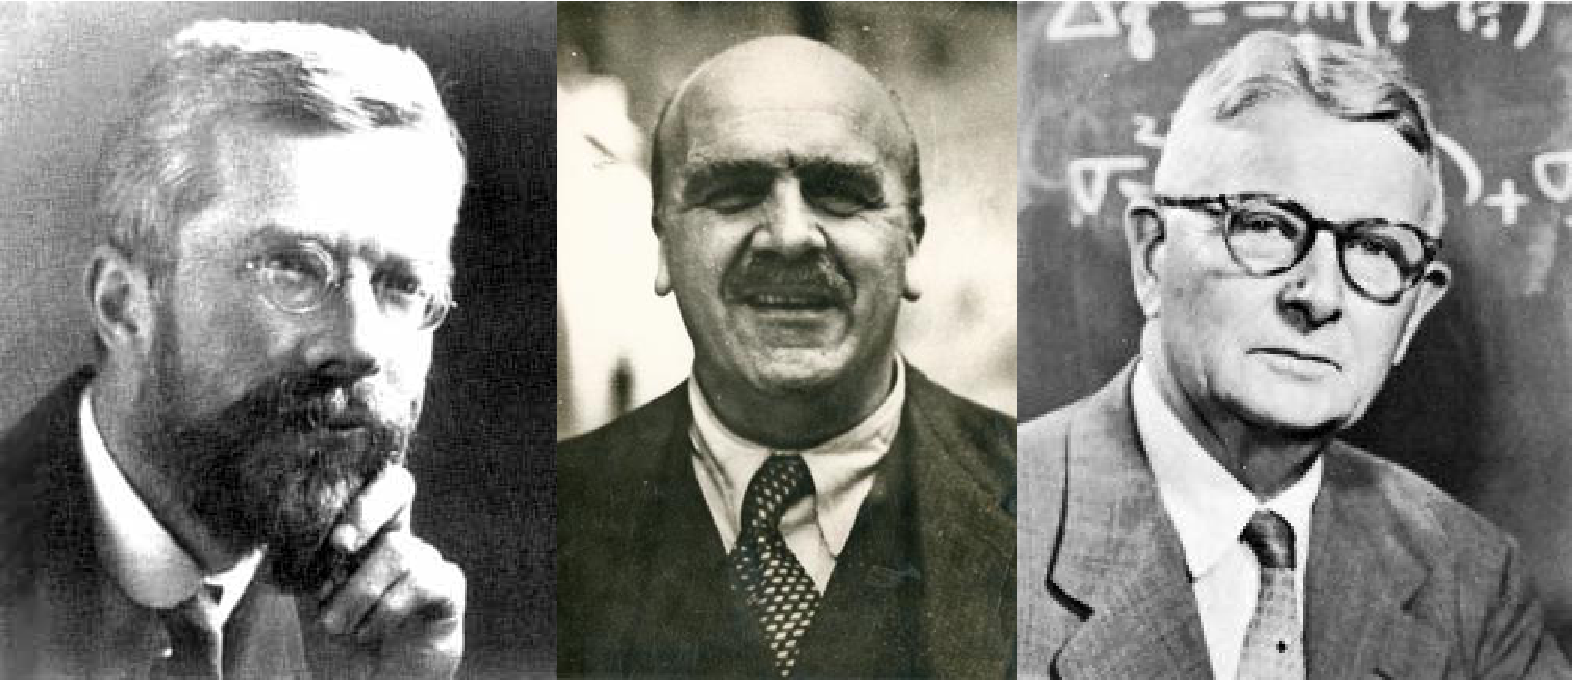
\includegraphics[width=0.75\textwidth]{fig/fisher-haldane-wright}
	\end{center}
	
\end{frame}

%%
\subsection{Empirical motivation}
%%

\begin{frame}[t]{Empirical motivation}
	There was a particularly fruitful synergism between the theoretical and empirical work being done for polyploids during the Modern Synthesis.
	\vspace{0.1in}
	
	\begin{center}
		\includegraphics[width=\textwidth]{fig/barlow-mather}
	\end{center}
\end{frame}

\begin{frame}[c]{And of course...}
\framesubtitle{Barbara McClintock}

Work on polyploid \textit{Zea}.

	\begin{center}
		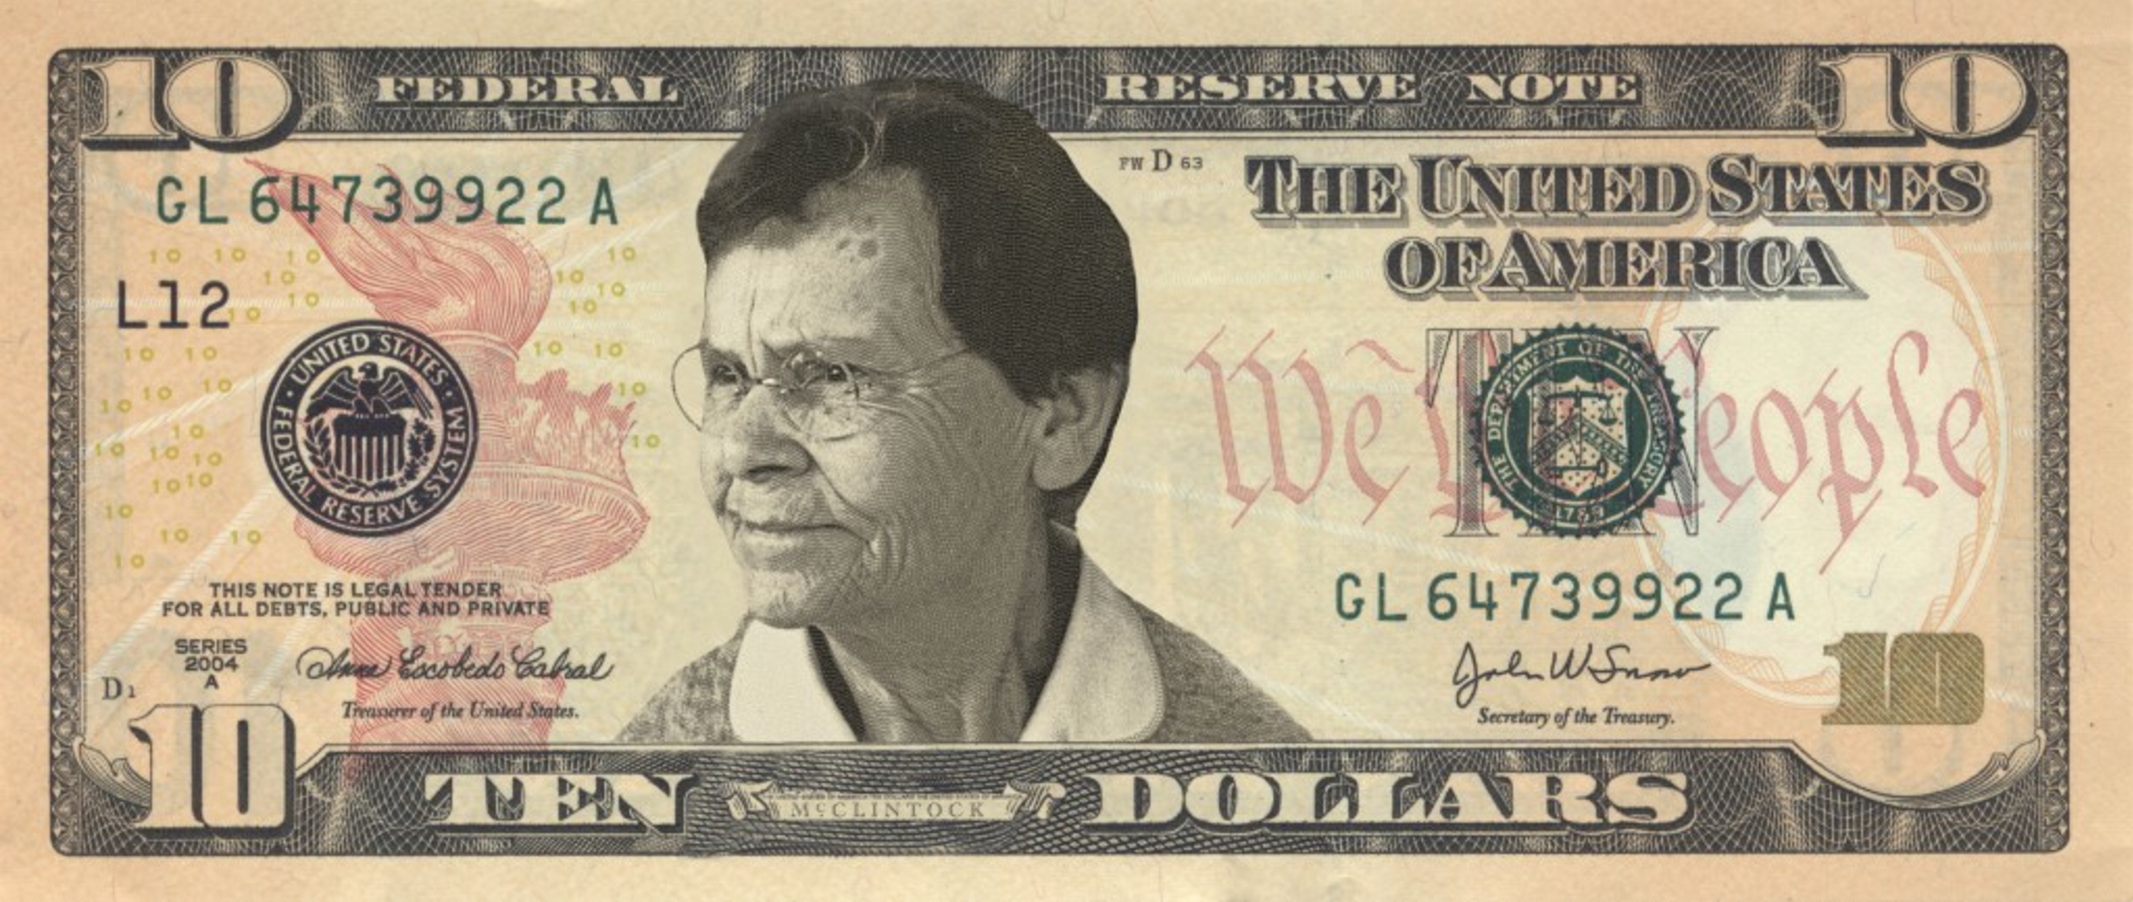
\includegraphics[width=\textwidth]{fig/barbara10}
	\end{center}
	
	\hfill {\scriptsize \#Barbara10}

\end{frame}

%%%%
\section{Polyploid pop-gen}
%%%%

%%
\subsection{Challenges}
%%

\begin{frame}[t]{Polyploid pop-gen}
\framesubtitle{Challenges}
	The difficulties of making population genetic inferences in polyploids present themselves at two broad levels:
	\vspace{0.1in}
	
	\begin{enumerate}
		\item \textbf{Allelic Dosage Uncertainty}: the inability to fully resolve the genotype of a partially heterozygous polyploid individual for a codominant marker (microsatellite, SNP).
		\vspace{0.2in}
		
		\item \textbf{Allelic inheritance}: disomic vs. polysomic vs. heterosomic, selfing, clonal, double reduction, etc.
	\end{enumerate}


\end{frame}

%%
\subsection{Allelic Dosage Uncertainty}
%%

\begin{frame}[t]{Allelic Dosage Uncertainty (ADU)}
	\textit{...the inability to fully resolve the genotype of a partially heterozygous polyploid individual for a codominant marker.}
	\vspace{0.1in}
	
	\begin{itemize}
		\item \textbf{Partial heterozygote} -- when the number of observed alleles at a locus is less than the ploidy level and not equal to 1 (i.e., is homozygous).
		\vspace{0.1in}

		\item \textbf{Ex}: For a locus with observed alleles A, B and C in a tetraploid (4N), the possible genotypes are AABC, ABBC or ABCC.
		\vspace{0.1in}
		
		\item The higher the ploidy, the worse the problem.
		\vspace{0.1in}
		
		\item Biallelic SNPs will always be partially heterozygous for a polyploid.
		
	\end{itemize}
	
\end{frame}

%%
\subsection{Overcoming ADU}
%%

\begin{frame}[t]{Overcoming ADU}
	For a biallelic locus, such as a SNP, we can use techniques like RAD sequencing to ``sample" from the genotype (model with binomial probability distribution*).
	\vspace{0.2in}
	
	\begin{center}
		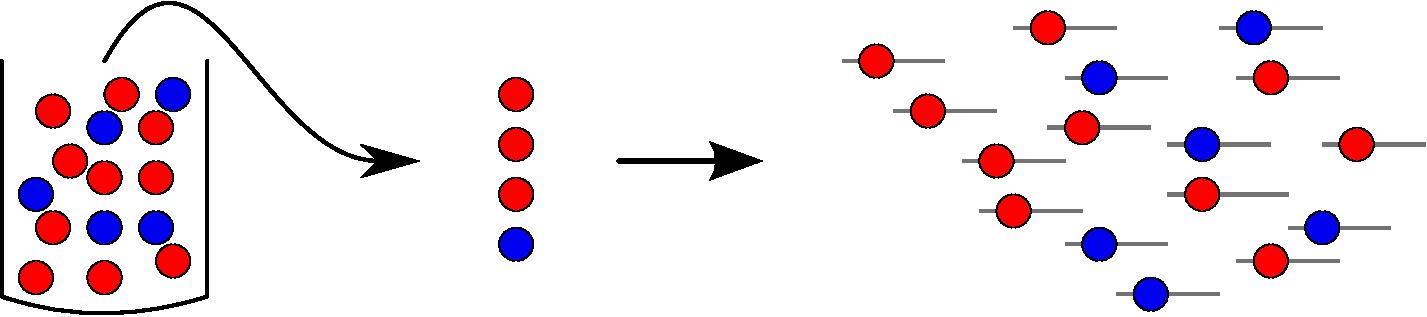
\includegraphics[width=\textwidth]{fig/pop-gen-model-empty}
	\end{center}
	
	\pause
	\begin{equation*}
	P(10 \text{ red reads}|k \text{ red alleles}) = \binom{16}{10}\left(\frac{k}{4}\right)^{10}\left(1-\frac{k}{4}\right)^6
	\end{equation*}
	
\end{frame}

\begin{frame}[t]{Overcoming ADU}
	For a biallelic locus, such as a SNP, we can use techniques like RAD sequencing to ``sample" from the genotype (model with binomial probability distribution*).
	\vspace{0.2in}
	
	\begin{center}
		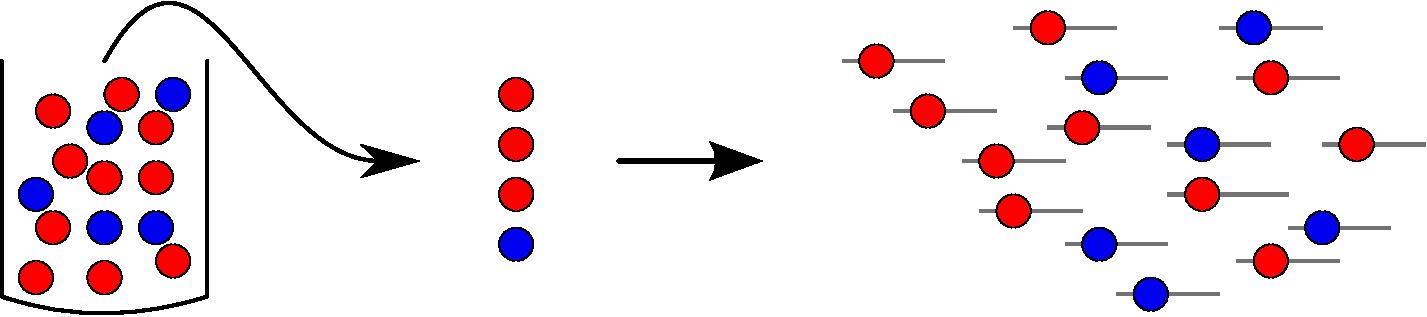
\includegraphics[width=\textwidth]{fig/pop-gen-model-empty}
	\end{center}

	\vspace{0.1in}
	Let's translate the entire illustration into something more mathematical.
\end{frame}

\begin{frame}[c]{A hierarchical model for polyploids}
	$p_{\ell}$ -- allele frequency at locus $\ell$. \\
	$g_{i \ell}$ -- genotype for individual $i$ at locus $\ell$. \\
	$r_{i \ell}$ -- sequencing reads for individual $i$ at locus $\ell$.
	\vspace{0.1in}
	\begin{center}
		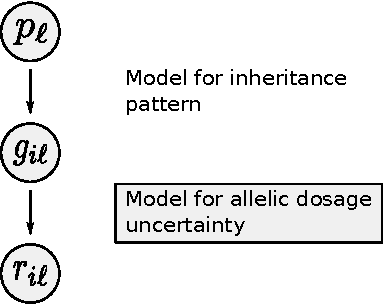
\includegraphics[width=0.6\textwidth]{fig/figure1-model-graph}
	\end{center}
\end{frame}

\begin{frame}[t]{A hierarchical model for polyploids}
	\fontsize{10pt}{10}\selectfont
	\vspace{-0.21in}
	\begin{align*}
		P(\text{allele freq} \vert \text{sequencing reads}) \propto\, \sum_{\text{genos}} &P(\text{sequencing reads} \vert \text{genotype}) \times\\
		&P(\text{genotype} \vert \text{allele freq})P(\text{allele freq})
	\end{align*}
		
	\begin{center}
		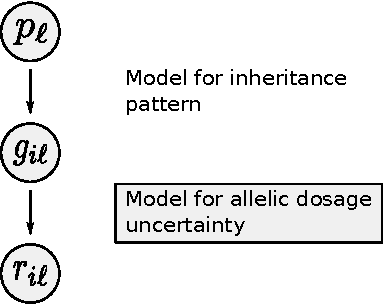
\includegraphics[width=0.6\textwidth]{fig/figure1-model-graph}
	\end{center}
\end{frame}

%%%%
\section{Simulations}
%%%%

%%
\subsection{Setup}
%%

\begin{frame}[t]{Simulations}
	\framesubtitle{Setup}
	
	We used the following settings for the simulations to test our model:
	\vspace{0.1in}
	
	\begin{itemize}
		\item Tetraploids (4N) and hexaploids (6N).
		\item Allele frequencies: 0.01, 0.05, 0.1, 0.2, 0.4.
		\item Sequencing coverage (average \# of reads per individual per locus): 5x, 10x, 20x, 50x, 100x.
		\item Number of individuals sampled: 5, 10, 20, 30.
	\end{itemize}
\end{frame}

%%
\subsection{Results}
%%

\begin{frame}[c]{Results}
	\framesubtitle{Heatmaps}
	\textbf{x-axis}: \# of individuals, \textbf{y-axis}: coverage, \textbf{scale}: error (s.d.)
	\pause
	\begin{center}
		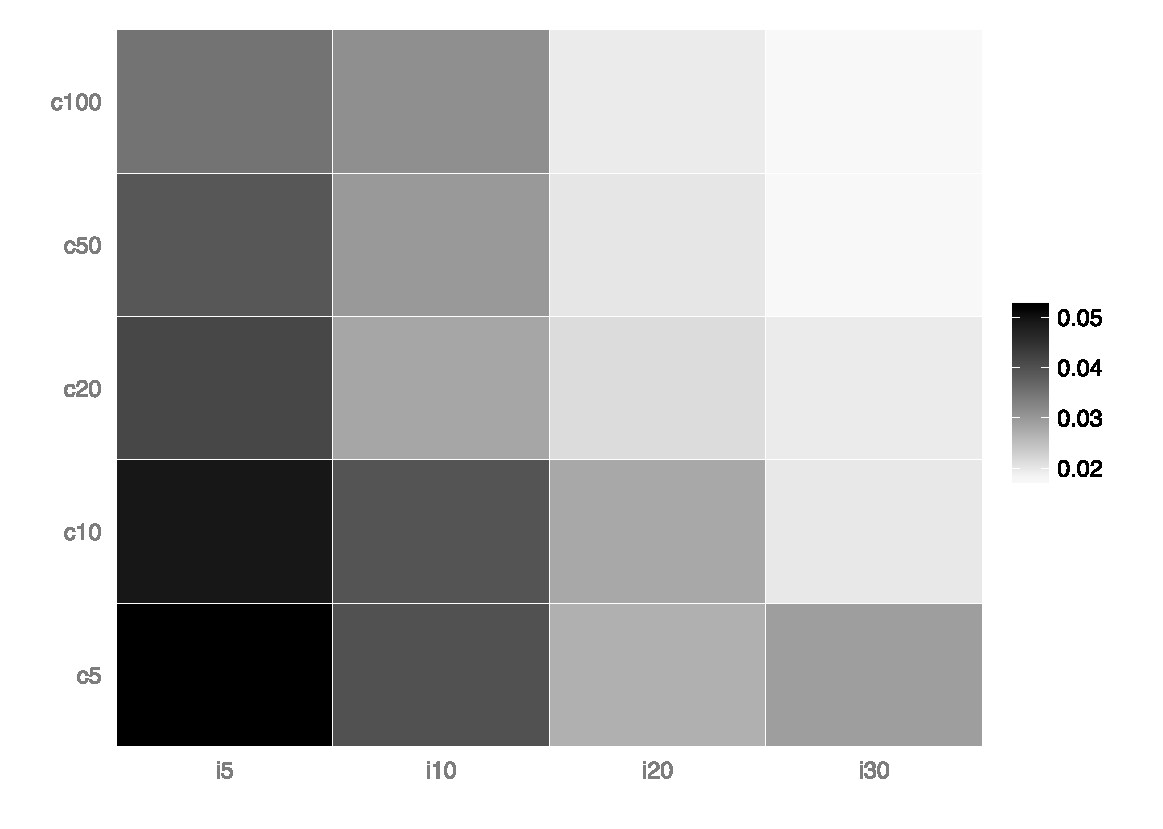
\includegraphics[width=0.85\textwidth]{fig/hex-plot0-05}
	\end{center}
\end{frame}

\begin{frame}[c,plain]{}
	\begin{center}
		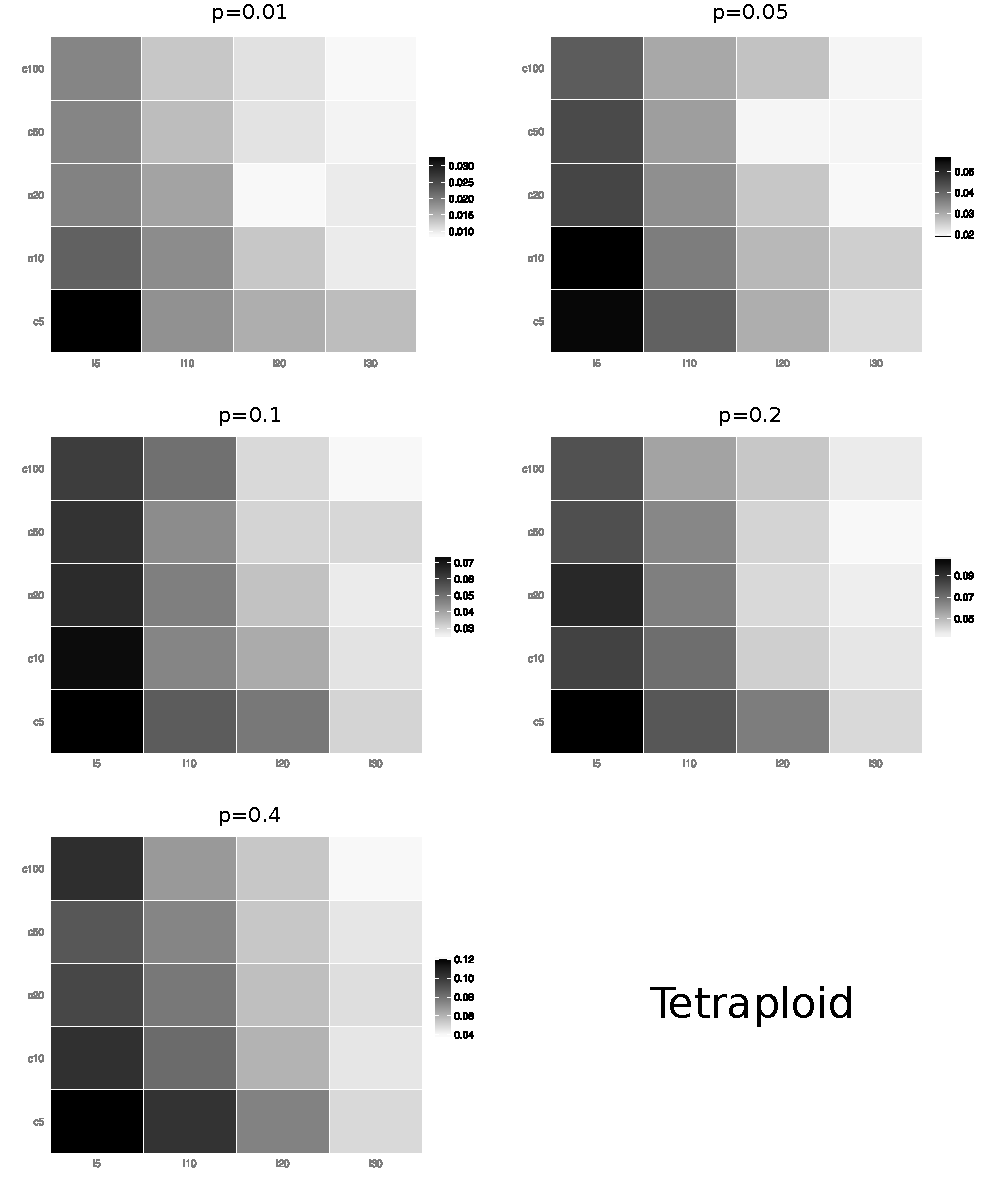
\includegraphics[width=0.7\textwidth]{fig/figure2-tetra-heatmaps}
	\end{center}
\end{frame}

\begin{frame}[c,plain]{}
	\begin{center}
		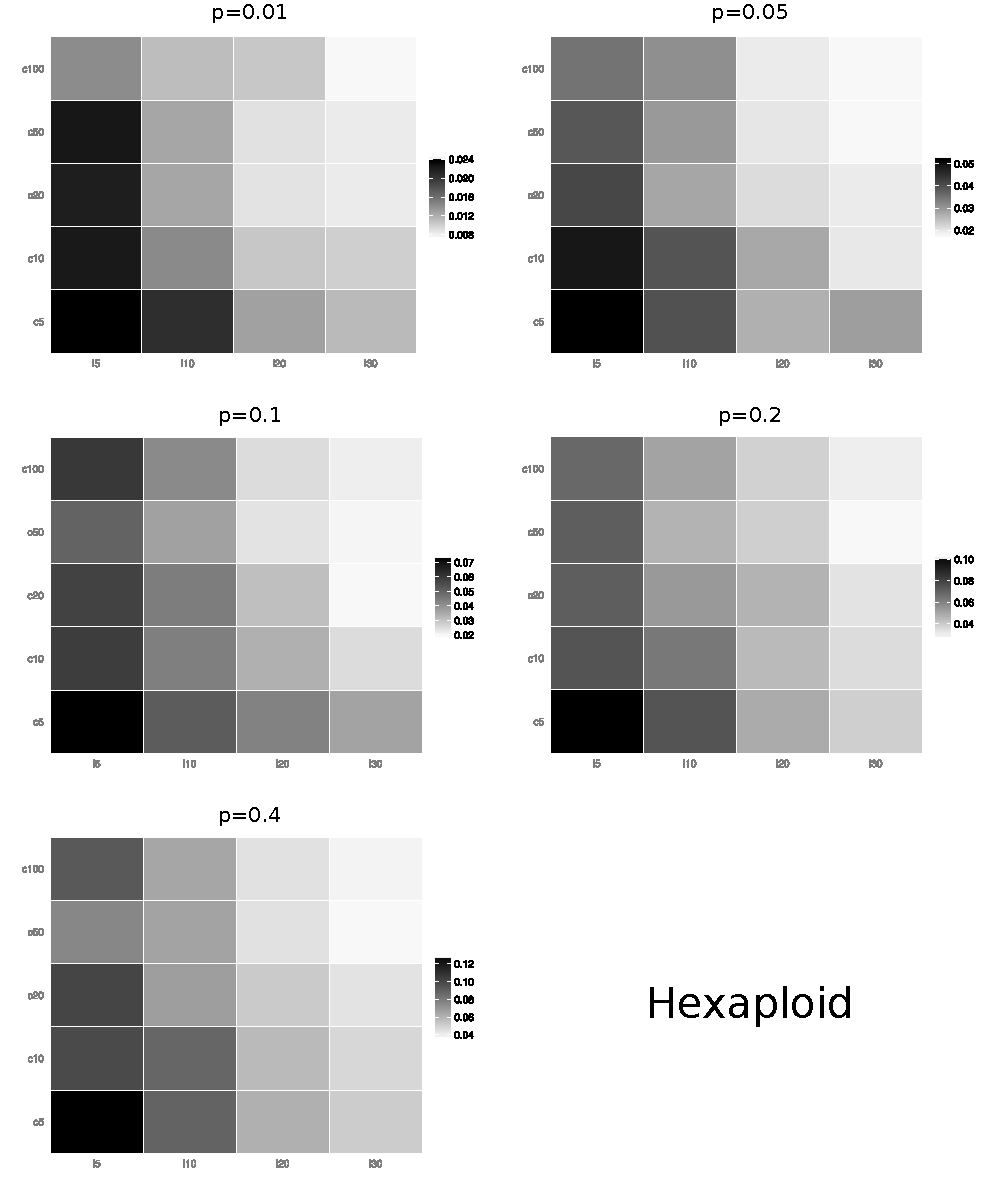
\includegraphics[width=0.7\textwidth]{fig/figure3-hex-heatmaps}
	\end{center}
\end{frame}

%%%%
\section{Conclusions}
%%%%

\subsection*{Conclusions}

\begin{frame}[t]{Conclusions}
	\fontsize{10pt}{10}\selectfont
	\begin{itemize}
		\item \textsc{Take home}: \textbf{Don't have to use genotypes as the first line of data}. Using sequencing reads is a viable solution for dealing with ADU.
		\vspace{0.2in}
	
		\item \textbf{The framework presented here is highly extensible}. Future work includes generalizing to both auto- and allopolyploids, more complex patterns of inheritance.
		\vspace{0.2in}
		
		\item \textbf{Sampling more individuals appears to be most important}. More individuals over higher sequencing coverage.
		\vspace{0.2in}
		
		\item \textbf{Need empirical data}. Simulations are nice, but we need to see how a model such as this works for lab-collected data.
		
	\end{itemize}
	
\end{frame}

%%%%
\section*{}
%%%%

\begin{frame}[t,plain]{Code availability}
	\fontsize{10pt}{10}\selectfont
	\begin{itemize}
		\item \textbf{polyfreqs}: an R package for the estimation of allele frequencies in autopolyploids. Available on GitHub -- \url{https://github.com/pblischak/polyfreqs}.
		\vspace{0.2in}
		
		\item Manuscript is currently in review, preprint is on bioR$\chi$iv -- \url{http://biorxiv.org/content/early/2015/07/02/021907}.
		\vspace{0.2in}
	
		\item Data and code for the simulation study and making the figures are on GitHub -- \url{https://github.com/pblischak/polyfreqs-ms-data}.
		\vspace{0.2in}
	
		\item Presentation slides are on fig\textbf{share}, and the \LaTeX{} source code is also on GitHub -- \url{https://github.com/pblischak/botany2015}.
	\end{itemize}
	\vspace{0.15in}
	
	{\Large \alert{All these links are in the GitHub repository for this presentation: \textbf{pblischak/botany2015}.}}
	
	\hfill {\tiny \#openscience}
\end{frame}

\begin{frame}[t,plain]{Acknowledgments}
	\begin{columns}[onlytextwidth]
	\column{0.4\textwidth}
	\begin{itemize}
		\item Aaron Wenzel, and members of the Wolfe and Kubatko labs.
		\item Ohio Supercomputer Center (Simulations).
		\item American Society of Plant Taxonomists (Travel Award).
		\item National Science Foundation (Funding).
	\end{itemize}
	
	\column{0.4\textwidth}
	\begin{center}
	
\includegraphics[width=0.85\textwidth]{fig/logos}
	\end{center}
	\end{columns}
\end{frame}

\begin{frame}[c,plain]{}
	\begin{center}
		{\Huge Thanks!}\\
		\vspace{0.5in}
		{\LARGE Questions?}
	\end{center}
\end{frame}

\end{document}